
\documentclass[letterpaper]{report}

\usepackage{listings}
\usepackage{graphicx}


\newenvironment{exercise}[1]
{\par\vspace{12pt}\noindent\textbf{Exercise \footnotesize{(#1)}}\\\begin{itshape}\begin{small}\noindent}
{\end{small}\end{itshape}}

\title{Zoltar Tutorial}
\date{}
\author{Tom Janssen\\
	December 17, 2009\\
	Software Technology Department\\
	Delft University of Technology}

\begin{document}

\maketitle{}
\lstset{language=C, 
		basicstyle=\small, 
		frame=single, 
		frameround=tttt,
		numbers=left, 
		numberstyle=\tiny, 
		xleftmargin=0cm, 
		xrightmargin=0cm,
		float=h!}

		
\begin{abstract}

Zoltar is a toolset for automatic software fault localization developed at 
the Software Technology Department of the Delft University of Technology.
It provides the means to automatically instrument source code of various types of software
in order to produce runtime information that is analyzed using 
a spectrum-based fault localization technique to produce a ranked list of likely faulty locations.
This tutorial provides the necessary information to be able to install, use and improve on the
Zoltar toolset.
\end{abstract}


\tableofcontents{}


%---------------------------------------------------------------------------------
\chapter*{Acknowledgements}
The author would like to express his gratitude to prof. dr. ir. Arjan van Gemund and
dr. Rui Maranhao for their guidance in writing this tutorial.
Sincere gratitude also goes to the Embedded Systems Institute (ESI), especially
to Hristina Moneva and Jozef Hooman for their reviews and advise.


%---------------------------------------------------------------------------------
\chapter{Introduction}
\label{c:Introduction}


Debugging is an important part of software development.
Several debugging tools exist which are based on stepping through the execution of the program.
These tools require the user to have knowledge about the code that is executed and 
about the inner workings and dependencies in the program 
which can be very difficult for one person to comprehend.

In practice, a large test set usually exists against which the program under development is tested.
Some tests will fail, some will pass, and this information can indicate what is going wrong
when unexpected behavior occurs.
However, in many cases, especially for large programs, 
a tester needs extensive knowledge about the program to be able to 
map a certain output or behavior to a point in the source code.

% With different testing and debugging methods available, 
% still there are times at which it is uncertain which locations of the source code should be investigated.
% These moments of undecidability can cause a great delay in software development
% and can limit the completeness and the stability of the product,
% given the relatively short time-to-market these days.

A solution to these issues would be a black box method 
which takes a program and available test cases 
and returns the most probable location of the fault
in case a number of these tests fail.
% In this tutorial a set of tools is introduced and explained
% which is able to do just that.
In this tutorial a toolset is introduced that implements
a technique called Spectrum-based Fault Localization (SFL \cite{sfltaicpart}).
SFL is based on instrumenting a program and keeping track of executed parts of the code
after which the spectrum-based fault localization technique is applied to 
return a list of source code locations ordered by the likelihood of it containing the fault.
Furthermore, the tool set enables a program to be trained with expected behavior
and to automatically detect an error if it encounters unexpected behavior.
The fact that no knowledge is needed of the program to acquire possible fault locations
would make this set of tools a useful extension to 
currently applied methods of testing and debugging.

The toolset is called \textsc{Zoltar}
%\footnote{\textsc{Barinel} stands
%for Bayesian AppRoach to dIagnosing iNtErmittent fauLts. A barinel is a type
%of caravel used by the Portuguese sailors during their discoveries.}
and is the result of research done at TUD in the context
of the TRADER project~\cite{trader},
involving several Dutch universities, Philips Tass, IMEC, and NXP
Semiconductors and is conducted under the
responsibility of the Embedded Systems Institute (ESI) in Eindhoven, the
Netherlands. The main goal of the
TRADER project was to develop methods and tools for ensuring reliability
of consumer electronic
products, minimizing product failures that are exposed to the end user.

This tutorial is organized as follows.
Chapter \ref{c:SFL} gives background information on the spectrum-based fault localization
technique which is adopted by the Zoltar toolset.
In Chapter \ref{c:Installation} the installation of the tools is explained
and the different tools of the package are discussed.
In Chapter \ref{c:ExampleProgramAnalysis} an example program is discussed
which is then instrumented and analyzed using the tools.
It will show the basics of the tools and enables the reader to perform
a quick program analysis.
Chapter \ref{c:ProgramSpectrumGeneration} gives some details of 
the instrumentation of program points which together will create program spectra.
Chapter \ref{c:AutomaticErrorDetection} contains information on 
the instrumentation, training and testing of a program in order to 
support automatic error detection.
The process of instrumentation is generalized in Chapter \ref{c:AnalyzingLargePrograms}
to be able to efficiently analyze large projects consisting of multiple source files.
Chapter \ref{c:BatchExecution} contains information on options in the tools to aid in
batch execution of tests.
Finally, the appendices contain detailed information of techniques and developers information
for the tool set.


%---------------------------------------------------------------------------------
\chapter{Spectrum-based Fault Localization}
\label{c:SFL}


% excerpt of TAIC PART

An important part of diagnosis and repair consists in
localizing faults.
Several tools for automated 
debugging and systems diagnosis implement an approach
to fault localization based on an analysis of the 
differences in program \emph{spectra} for \emph{passed} and \emph{failed}
runs. Passed runs are executions of a program that
are completed correctly, whereas failed runs are executions
in which an error was detected. A program spectrum is
an execution profile that indicates which parts of a 
program are active during a run. Fault localization entails
identifying the part of the program whose activity 
correlates most with the detection of errors. 

Spectrum-based fault localization (SFL) does not rely on
a model of the system under investigation. It can easily 
be integrated with existing testing procedures, and
because of the relatively small overhead with respect
to CPU time and memory requirements, it lends itself
well for application within resource-constrained 
environments. However, the efficiency of 
SFL comes at the cost of a limited
diagnostic accuracy. 
As an indication, in one of the 
experiments described in 
\cite{sfltaicpart}, 
on average
20\% of a program still needs to be inspected after the
diagnosis.

\section{Failures, Errors, and Faults}
\label{s:failuresErrorsFaults}
A \emph{failure} is an event that occurs when delivered service
deviates from correct service. An \emph{error} is a system
state that may cause a failure. A \emph{fault} is the cause of
an error in the system.
Since we focus on computer programs, faults are bugs in the program code, and failures occur
when the output for a given input deviates from the
specified output for that input.

\newpage

\lstinputlisting
	[captionpos=b, label=l:rationalSort, caption=A faulty C function for sorting rational numbers.]
	{sources/RationalSort_snippet.c}
	
To illustrate these concepts, consider the C 
function in Listing \ref{l:rationalSort}. 
It is meant to sort, using the 
bubble sort algorithm, a sequence of \verb|n| rational numbers
whose numerators and denominators are stored in the
parameters \verb|num| and \verb|den|, respectively. There is a fault
(bug) in the swapping code within the body of the if
statement: only the numerators of the rational 
numbers are swapped while the denominators are left in
their original order. In this case, a failure occurs
when \verb|RationalSort| changes the contents of its 
argument arrays in such a way that the result is not a
sorted version of the original. An error occurs after
the code inside the conditional statement is executed,
while \verb|den[j]| $\neq$ \verb|den[j+1]|. Such errors can be 
temporary, and do not automatically lead to failures. For
example, if we apply RationalSort to the sequence
$\langle \frac{4}{1}, \frac{2}{2}, \frac{0}{1} \rangle$,
an error occurs after the first two 
numerators are swapped. However, this error is "canceled" by
later swapping actions, and the sequence ends up being
sorted correctly.

Error detection is a prerequisite for SFL: we must know
that something is wrong before we can try to locate
the responsible fault. Failures constitute a 
rudimentary form of error detection, but many errors remain
latent and never lead to a failure. An example of a
technique that increases the number of errors that can
be detected is array bounds checking. Failure 
detection and array bounds checking are both examples of
generic error detection mechanisms, that can be 
applied without detailed knowledge of a program. Other
examples are the detection of null pointer handling,
malloc problems, and deadlock detection in concurrent
systems. Examples of program specific mechanisms are
precondition and postcondition checking, and the use
of assertions.

The Barinel toolset supports instrumenting for 
automatic error detection, which will be discussed in
Chapter \ref{c:AutomaticErrorDetection}.

\section{Program Spectra}
A program spectrum is a collection of data that
provides a specific view on the dynamic behavior of
software. This data is collected at run-time, and 
typically consist of a number of counters or 
flags for the
different parts of a program. Many different forms of
program spectra exist, some of which are supported by the Barinel toolset. 
In this example
we work with so-called block hit spectra.

A block hit spectrum contains a 
flag for every block
of code in a program, that indicates whether or not that
block was executed in a particular run. With a block of
code we mean a C language statement, where we do not
distinguish between the individual statements of a 
compound statement, but where we do distinguish between
the cases of a switch statement. As an illustration, we
have identified the blocks of code in Listing \ref{l:rationalSort}.


\section{Fault Localization}
The hit spectra of \emph{N} runs constitute a binary matrix,
whose columns correspond to \emph{M} different parts (blocks
in our case) of the program. The 
information in which runs an error was detected 
constitutes another column vector, the error vector. This
vector can be thought to represent a hypothetical part
of the program that is responsible for all observed 
errors. 
This is visualized in Figure \ref{fig:Ae}.
Fault localization essentially consists in 
identifying the part whose column vector resembles the error
vector most.

\begin{figure}[h!]
	\begin{center}
	\begin{tabular}{c c c}
							&					& error \\
							& $M$ components	& detection \\
			$N$ spectra 	& 
		$ \left[
		\begin{array}{c c c c}
			a_{11} & a_{12} & \ldots & a_{1M} \\
			a_{21} & a_{22} & \ldots & a_{2M} \\
			\vdots & \vdots & \ddots & \vdots \\
			a_{N1} & a_{N2} & \ldots & a_{NM} \\
		\end{array}
		\right] $
		&
		$ \left[
		\begin{array}{c}
			e_1 \\
			e_2 \\
			\vdots \\
			e_N \\
		\end{array}
		\right] $
		\\
	\end{tabular}
	\caption{Input to SFL}
	\label{fig:Ae}
	\end{center}
\end{figure}

In the field of data clustering, resemblances between
vectors of binary, nominally scaled data, such as the
columns in our matrix of program spectra, are 
quantified by means of similarity coefficients.
By default, the Barinel toolset uses the Ochiai coefficient
$s_O$, used in the molecular biology domain,
since this coefficient performed best in experiments
\cite{sfltaicpart}:\\
\begin{center}
$s_O(j) = \frac{n_{11}(j)}{\sqrt{(n_{11}(j)+n_{01}(j))*(n_{11}(j)+n_{10}(j))}}$\\
\end{center}
where $n_{pq}(j)$ indicates the number of runs in which block \emph{j} 
has been touched during the execution, denoted by $p \in \{0,1\}$,
and where the runs are failed or passed, indicated by $q \in \{0,1\}$:
\begin{center}
\begin{tabular}{c|c|c}
$n$ & touched & run \\
\hline
$n_{00}$ & no & passed \\
$n_{10}$ & yes & passed \\
$n_{01}$ & no & failed \\
$n_{11}$ & yes & failed \\
\end{tabular}
\end{center}

Under the assumption that a high similarity to the
error vector indicates a high probability that the corresponding parts of the software cause the detected
errors, the calculated similarity coefficients rank the
parts of the program with respect to their likelihood of
containing the faults.

To illustrate the approach, suppose that we 
apply the \verb|RationalSort| function to the input sequences
$I_1$, \ldots ,$I_6$ (see below). The block hit spectra for these
runs are as follows ('1' denotes a hit), where block 5
corresponds to the body of the \verb|RationalGT| function,
which has not been shown in Listing \ref{l:rationalSort}.
\begin{center}
\begin{tabular}{l|c c c c c|c}
\multicolumn{1}{c}{} & \multicolumn{5}{c}{block} & \\
input & 1 & 2 & 3 & 4 & 5 & error \\
\hline
$I_1 = \langle \rangle$ 
& 1 & 0 & 0 & 0 & 0 & 0 \\
$I_2 = \langle \frac{1}{4} \rangle$ 
& 1 & 1 & 0 & 0 & 0 & 0 \\
$I_3 = \langle \frac{2}{1}, \frac{1}{1} \rangle$ 
& 1 & 1 & 1 & 1 & 1 & 0 \\
$I_4 = \langle \frac{4}{1}, \frac{2}{2}, \frac{0}{1} \rangle$ 
& 1 & 1 & 1 & 1 & 1 & 0 \\
$I_5 = \langle \frac{3}{1}, \frac{2}{2}, \frac{4}{3}, \frac{1}{4} \rangle$ 
& 1 & 1 & 1 & 1 & 1 & 1 \\
$I_6 = \langle \frac{1}{4}, \frac{1}{3}, \frac{1}{2}, \frac{1}{1} \rangle$ 
& 1 & 1 & 1 & 0 & 1 & 0 \\
\hline
\multicolumn{1}{c|}{$s_O$} & $.40$ & $.44$ & $.50$ & $.58$ & $.50$ & \\
\end{tabular}
\end{center}

$I_1$, $I_2$, and $I_6$ are already sorted, and lead to passed
runs. $I_3$ is not sorted, but the denominators in this
sequence happen to be equal, hence no error occurs. $I_4$
is the example from Section \ref{s:failuresErrorsFaults}: 
an error occurs during
its execution, but goes undetected. For $I_5$ the program
fails, since the calculated result is 
$\langle \frac{1}{1}, \frac{2}{2}, \frac{4}{3}, \frac{3}{4} \rangle$
instead of 
$\langle \frac{1}{4}, \frac{2}{2}, \frac{4}{3}, \frac{3}{1} \rangle$
, which is a clear indication that an error
has occurred. For this data, the calculated similarity
coefficient $s_O$ (correctly)
identifies block 4 as the most likely location of the fault.
In general, however, the faulty component(s) may be outranked
by other components, entailing non-zero search effort by the users.
Research has shown that for small programs ($O(100)$ lines) 
$5 - 20 \%$ of the code remains to be inspected by the user \cite{ZAGGECBS:07}.
However, for large programs this fraction drops to less than a percent \cite{ijcai09},
making SFL an interesting debugging aid.



%---------------------------------------------------------------------------------
\chapter{Installation}
\label{c:Installation}


The Zoltar tool set depends on the Low Level Virtual Machine framework and
is currently only known to be compatible with version 2.4.
This version of \verb|llvm| can be downloaded from 
\verb|http://llvm.org| and can be installed according to their instructions.
Also, make sure the \verb|ncurses| and \verb|libgtk-2.0dev| packages are
installed on your system.
At the time of writing this tutorial, the tools are only tested on linux (Ubuntu and Fedora).

\section{Installing llvm}
The following shows an example of installing the \verb|llvm| tools.
This serves as a guideline to quickly get a working toolset,
but does not cover all details and is not guaranteed to work on your system.
It is recommended to look at the getting-started guide on the \verb|llvm| website:\\
\verb|  http://llvm.org/docs/GettingStarted.html|

First, download the \verb|llvm| version 2.4 sources and the
\verb|llvm-gcc frontend| sources.
The latter is required to compile C programs using \verb|llvm|.
Both are located at\\
\verb|  http://llvm.org/releases/download.html#2.4|\\
Next, unpack both using\\
\verb|  # tar -xzf llvm-2.4.tar.gz|\\
\verb|  # tar -xzf llvm-gcc-4.2-2.4.source.tar.gz|\\
Make an object directory and an install directory for llvm:\\
\verb|  # mkdir llvm-obj|\\
\verb|  # mkdir llvm-install|\\
Install \verb|llvm|:\\
\verb|  # cd llvm-obj|\\
\verb|  # ../llvm-2.4/configure|\\
\verb|  # make|\\
At this point, an \verb|llvm| version without gcc-frontend is built.
To make the gcc-frontend, however, we need this installation of \verb|llvm|.
Make an object directory and an install directory for \verb|llvm-gcc| as well:\\
\verb|  # cd ..|\\
\verb|  # mkdir llvm-gcc-obj|\\
\verb|  # mkdir llvm-gcc-install|\\
and configure it to use the \verb|llvm| we have just installed.\\
\verb|  # cd llvm-gcc-obj|\\
\verb|  # ../llvm-gcc4.2-2.4.source/configure \ |\\
\verb|  > --prefix=`pwd`/../llvm-gcc-install --program-prefix=llvm- \ |\\
\verb|  > --enable-llvm=`pwd`/../llvm-obj --enable-languages=c,c++ |\\
\verb|  # make|\\
\verb|  # make install|\\
After this, \verb|llvm| must be reconfigured to include \verb|llvm-gcc|.\\
\verb|  # cd ../llvm-obj|\\
\verb|  # ../llvm-2.4/configure --prefix=`pwd`/../llvm-install \ |\\
\verb|  > --withllvmgccdir=`pwd`/../llvm-gcc-install|\\
\verb|  # make |\\
\verb|  # make install |

The above procedure will have created two installation directories,
\verb|llvm-install| and \verb|llvm-gcc-install|.
The \verb|bin| directories of both should be in the \verb|PATH| environment,
enabling a system wide call to the \verb|llvm| tools.


\section{Installing Zoltar}

The source package can be downloaded from \verb|http://fdir.org|.
Unpack it with \\
\verb|  # tar -xzf zoltar.tar.gz|\\
Inside the unpacked directory run \\
\verb|  # ./configure --with-llvmsrc=<LLVMSRCDIR> \|\\
\verb|  > --with-llvmobj=<LLVMOBJDIR> --prefix=<INSTALLDIR>|\\
where \verb|<LLVMSRCDIR>| and
\verb|<LLVMOBJDIR>| should be the directory containing the 
\verb|llvm| source files and \verb|llvm| object files respectively
(\verb|/path/to/llvm-2.4| and \verb|/path/to/llvm-obj| in the previous section).
\verb|<INSTALLDIR>| should be the place where you want the tool binaries and libraries to
be located.
Next, build and install the tool set using \\
\verb|  # make|\\
\verb|  # make install|\\
At this point the Zoltar tools are installed in the \verb|bin| directory of \verb|<INSTALLDIR>|
and the libs are installed in the \verb|lib| directory.
Make sure to include the \verb|bin| directory in the \verb|PATH| environment 
and to include the \verb|lib| dir in the library search path (using libtool) or, alternatively,
using the \verb|-L/path/to/lib| option during linking, or
copy the \verb|*.so*| files to a library search path, such as \verb|/usr/lib|
(this is not recommended and is not seen as a general solution, though).
In the remainder of the tutorial it is assumed that the linker can find the libraries.

The resulting libraries and binaries are given in Table \ref{t:LibsAndTools} 
along with a short description.

\begin{table}
  \begin{tabular}{l|l}
    \hline
	\verb|libinstrument| & library which should be linked to the instrumented program \\
	\verb|libpasses|     & library with instrumentation passes loaded by the \verb|instrument| tool \\
	\verb|instrument|    & instrumentation tool \\
	\verb|zoltar|       & console based program analysis and configuring tool \\
	\verb|xzoltar|      & source code visualization of program analysis \\
    \hline
  \end{tabular}
  \caption{Description of libraries and tools}
  \label{t:LibsAndTools}
\end{table}


\section{Development Build}
  
To enable development of the Zoltar tools a debug installation is available.
This will enable debugging context to be compiled within the binaries and libraries,
which will aid in developing and debugging the toolset.
To build the debug version of the Zoltar tool set
also \verb|llvm| needs to be built in debug mode.
To do this, add the \verb|ENABLE_OPTIMIZED=0| option to the \verb|make|
commands while building the final version of \verb|llvm| (with llvm-gcc linked).\\
\verb|  # make ENABLE_OPTIMIZED=0| \\
\verb|  # make install ENABLE_OPTIMIZED=0| \\
This debug install procedure has then be done for the Zoltar toolset as well.
Note that \verb|llvm| has to be built in debug mode before building Zoltar in debug mode,
since the latter requires certain libraries of the debug installation of \verb|llvm|.

Within the directory of each tool or library in the Zoltar package one can type
\verb|make| to build a release version of that particular tool or library or type
\verb|make ENABLE_OPTIMIZED=0| to build a debug version.



 
%---------------------------------------------------------------------------------
\chapter{Example Program Analysis}
\label{c:ExampleProgramAnalysis}


In this chapter an example program will be introduced
which will be used to explain the use of the program analysis tools.
The basic routine of instrumentation, testing and analyzing will be discussed
to get acquainted with the tool set.


\section{Example Program}
\label{s:exampleProgram}

An example program called \verb|textVal| has been created to output some value based on an input text.
The value is calculated in the following way. 
For each letter of the alphabet the value is incremented by one,
for each digit the value is incremented by two
and for any other printable, non-space character the value is increased by ten.
This is according to the following equation.
\begin{center}
\begin{tabular}{rl}
$l =$ & number of letters  \\
$d =$ & number of digits \\
$o =$ & number of other characters \\
$v =$ & $ l + 2*d + 10*o $ \\
\end{tabular}
\end{center}

For demonstration purposes this program is deliberately created using three separate threads,
each scanning for a different sort of character and incrementing a shared value.
The complete source code is given in Listing \ref{l:textVal}.
Two bugs are introduced, which relate to mutual exclusion.
The critical section of this code is at the \verb|updateVal| function,
which adds the value of its argument to the shared value containing the result of the program.
The thread that is responsible for reading letters of the alphabet,
running the \verb|readLetters| function,
correctly locks the mutex.
However it is assumed that other threads do the same,
which is not always the case and which in practice results in hard to find bugs.
In this case, the thread that scans for digits (\verb|readDigits|) does not lock and unlock the mutex,
which results in a critical section that is not exclusively executed by one thread at a time.
If the first thread reads the shared value at line 16 and 
the second thread reads the same value before the first thread has written a value back,
then information is lost and the resulting value will be lower than expected.

The second introduced bug in this code is located in the code of the third thread,
which scans for special characters
using the function \verb|readOthers|.
This thread does lock the mutex, but does not release the exclusive right to the critical section,
resulting in a situation in which the first thread waits forever for the mutex to become unlocked.

\lstinputlisting
	[label=l:textVal, caption=source code for the textVal example program]
	{sources/textVal.c}

In the next sections an example analysis is made for the \verb|textVal| program.
In order to analyze the program we first have to instrument the code to 
have it keep a record of executed portions of code (a program spectrum).
This instrumented program is then run with different test inputs,
some resulting in correct output values, others failing to produce the correct value.
The data that is gathered during these tests is analyzed and 
this results in a list of possible locations of the fault.

	
\section{Instrumentation}
\label{s:instrumentation}
	
	First, the program has to be instrumented to create execution data during the tests.
	When running the instrumented program, 
	a counter corresponding to an instrumented piece of code is incremented 
	each time that piece of code is executed.
	This results in a spectrum of the execution of the program.
	
	Different types of program points can be instrumented.
	The tool set supports, for example, function level instrumentation
	and instrumentation at the basic block level, 
	but also supports custom instrumentations.
	Detailed information of instrumenting program points for creating
	program spectra is given in Chapter \ref{c:ProgramSpectrumGeneration}.
	
	Instrumentation is done by the \verb|instrument| tool.
	In our case we will instrument each basic block of the program.
	A basic block is defined as a sequence of statements with one entry point and one exit point,
	having no jump instructions contained within it.
	The following commands are used to instrument the program.\\
	\verb|  # llvm-gcc -g -emit-llvm -c textVal.c -o textVal.bc| \\
	\verb|  # instrument -f -spbasicblock -bypassmain -memprotection \ | \\
	\verb|  > textVal.bc -o textVal.ibc| \\
	\verb|  # llc -f textVal.ibc -o textVal.s| \\
	\verb|  # gcc textVal.s -lpthread -linstrument -o textVal| \\
	
	The first line uses the \verb|llvm-gcc| compiler to create \verb|llvm| \emph{intermediate byte code}.
	Care must be taken to include the \verb|-g| option to generate debug information,
	which is required during instrumentation.
	The \verb|-emit-llvm| and \verb|-c| options result in the creation of the byte code, 
	in stead of trying to create an executable.
	
	The second line is the actual instrumentation.
	The \verb|instrument| tool accepts multiple \emph{instrumentation passes},
	the \verb|-spbasicblock| pass being one of them.
	The \verb|-spbasicblock| option adds instrumentation of basic blocks.
	The \verb|-memprotection| option guarantees that the instrumented program
	will not be able to accidentally invalidate the data that is gathered during run-time.
	In order to achieve this, every store operation is checked to ensure it will not
	modify the part of memory which contains the instrumentation data.
	The \verb|-bypassmain| option bypasses the main function of the program,
	in order to initiate instrumentation data and to handle exceptions while
	not losing recorded data.
	Finally, the \verb|-f| option forces to overwrite existing output data.
	The output is an instrumented form of the \verb|llvm| byte code.
	
	The third line contains another \verb|llvm| tool to create native code from the 
	\verb|llvm| byte code.
	Again, the \verb|-f| option ensures that an existing output file is overwritten
	without complaining.
	
	The final line uses \verb|gcc| to link the resulting native code with 
	the \verb|pthread| library and with the \verb|instrument| library.
	The latter contains the functionality for initializing spectrum data,
	starting the instrumented program, handling spectrum updates and
	writing results into a datafile.
	
	At this point we have an executable program,
	which behaves as the original program would behave,
	with the added functionality of creating a program spectrum.
	In the next section we will create some test cases and 
	perform an analysis to locate the faults.
	

\section{Testing}

	In most software projects, tests are created along with the software itself.
	During the implementation and testing phases these tests are used to validate
	the functionality of the software.
	Failing tests indicate which features of the software are incomplete or faulty.
	However, software bugs are often not directly traceable to lines of code.
	Even test-driven implementation using unit tests will in many cases prove insufficient 
	to build bug free code.
	A piece of code can contain a fault which did cause an error in small tests
	but will lead to a failure when integrated into a larger code base.
	
	For the example program, a number of tests were created. 
	These include testing only letters for input, 
	only digits or special characters, or combinations of character types.
	These are standard tests to verify the functionality of the program.
	A problem in this case is that some small tests will work as expected,
	but will fail if they are scaled up.
	The mutex problem is the cause of this irregular behavior, 
	since task switching between the threads will unlikely occur 
	during the scanning of small input.
	
	\begin{table}
		\begin{center}
		\begin{tabular}{l|l|r r r|r|r}
			\hline
			          &       & \multicolumn{3}{c|}{summary} & expected & textVal \\
			test file & input & $l$ & $d$ & $o$ & output & output \\
			\hline
			test1.in & \verb|"abcdefghij"|   & $10$   & $0$   & $0$ & $10$   & $10$ \\
			test2.in & \verb|"0123456789"|   & $0$    & $10$  & $0$ & $20$   & $20$ \\
			test3.in & \verb|"A0B1C2D3E4"|   & $5$    & $5$   & $0$ & $15$   & $15$ \\
			test4.in & large text only       & $1040$ & $0$   & $0$ & $1040$ & $1040$ \\
			test5.in & large text and digits & $520$  & $200$ & $0$ & $920$  & $< 920$ \\
			test6.in & \verb|".=+-#"|        & $0$    & $0$   & $5$ & $50$   & hangs \\
		\end{tabular}
		\end{center}
		\caption{Test suite for the textVal program with information on the number of 
		letters, digits and other characters.}
		\label{t:TestSuite}
	\end{table}
	
	Table \ref{t:TestSuite} shows the test suite that is available for this program.
	The input, or a description of the input, is given 
	together with a summary in terms of the number of letters, digits and other characters.
	For each test also the expected output is given and the actual output of the program.
	
	First, test 1 to 5 are run, since test 6 shows different behavior than the incorrect output.
	These tests are run as follows.\\
	\verb|  # ./textVal < test1.in|\\
	\verb|  # ./textVal < test2.in|\\
	\verb|  # ./textVal < test3.in|\\
	\verb|  # ./textVal < test4.in|\\
	\verb|  # ./textVal < test5.in|\\
	You will see the correct output for the first four tests.
	Most likely, test 5 yields a value which is less than the expected value of 920.
	Test 6 results in the hanging of the program and will be discussed
	in Chapter \ref{c:AutomaticErrorDetection} (it should not yet be executed at this point).
	Note that, in practice, we have no real clue what the cause would be.
	We see that a text with mixed letters and digits works as expected,
	given that the size of the text is limited, but the same test fails if the text size is large.
	In conventional debugging one could be mislead by these results and would start looking at
	the text buffer or the reading of the input.
	In this case we use a black box method.
	A program is instrumented and run in the same way the original program would have been run.
	
	
\section{Analysis}

	The resulting run data of the test runs is stored in a separate file called \verb|datafile.dat|.
	This file is created after the first run and is incrementally updated at every next run.
	This data file contains program spectrum information, among other things.
	Before we can start the analysis using the \verb|zoltar| tool,
	first we need to specify which test runs have failed and which have passed.
	This can be done in two ways.
	The pass and fail information can be stored in a separate file, 
	containing a '1' for each passed test and a '0' for each failed test.
	This is very useful for running a batch of tests and is explained in Chapter \ref{c:BatchExecution}.
	The second method is through the \verb|zoltar| tool itself, 
	which is what will be shown next.
	
	The \verb|zoltar| tool can be started by typing\\
	\verb|  # zoltar|\\
	in the directory where the tests have been run.
	The \verb|datafile.dat| file is then automatically opened.
	The same holds for a context file called \verb|context.dat|.
	If the program has been instrumented in another directory the
	\verb|context.dat| file will be located in that directory.
	It contains the source file location for each instrumented program point
	to enable the mapping of probable fault locations in the executable 
	to the pieces of code in the original source file.
	In case the context file is located elsewhere, 
	the location can be passed with the following option.\\
	\verb|  # zoltar --contextfile=/path/to/context.dat|\\
	It might be wise to look at more options using the command:\\
	\verb|  # zoltar --help|\\
	Most options will be discussed in the remainder of this tutorial.
	
	When the tool is started the main menu is shown and is active.
	In the right hand window a summary of the instrumented program and the test runs is given,
	like the number of runs and the number of spectra that were instrumented.
	Changing the pass and fail information of the runs is done in the \verb|runs| submenu.
	This can be selected by pressing \emph{down} on the keyboard to navigate to the \verb|runs|
	entry in the main menu and by pressing \emph{enter}.
	The test runs are then listed and each run can be selected to change its status to \emph{passed}
	or \emph{failed}.
	In our case we will change the fifth run to \emph{failed}, 
	since the output of this run was not what we expected it to be.
	Figure \ref{fig:analyzeRuns} shows the screen of the \verb|zoltar| tool at this point.
	
	\begin{figure}[h!]
		\begin{center}
		\begin{tabular}{c}
			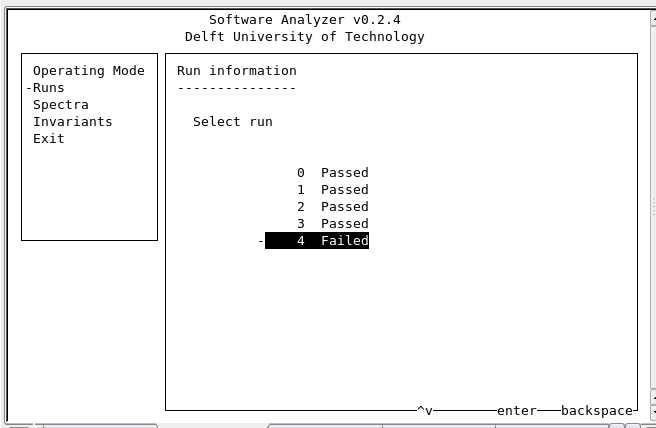
\includegraphics[scale=0.40]{sources/analyze_runs.png} \\
		\end{tabular}
		\end{center}
		\caption{The test run information of the textVal tests.}
		\label{fig:analyzeRuns}
	\end{figure}

	\begin{figure}[h!]
		\begin{center}
		\begin{tabular}{c}
			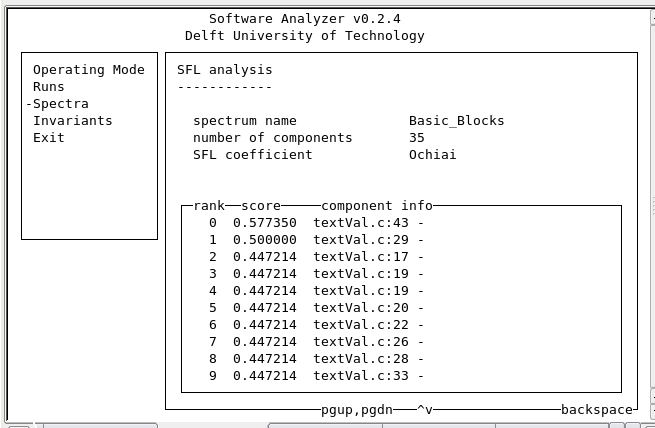
\includegraphics[scale=0.40]{sources/analyze_sfl.png} \\
		\end{tabular}
		\end{center}
		\caption{SFL results of the textVal tests.}
		\label{fig:analyzeSfl}
	\end{figure}
	
	The keys that can be used in each screen are shown at the bottom of the screen.
	To go back to the previous screen the '\emph{backspace}' key can be pressed.
	Back in the main menu the \verb|Spectra| entry can be chosen to investigate the
	program spectrum of the basic blocks, which we have created during the test runs.
	To do this, select the \verb|Spectra| entry, then select \verb|Basic Blocks| 
	in the \verb|select spectrum| screen.
	At this point we can choose to inspect the spectrum data 
	or perform SFL on the data.
	We will select the \verb|Perform SFL analysis| option and select the
	\verb|Ochiai| similarity coefficient.
	Other coefficients are also possible, but are present for research purposes.
	The \verb|Ochiai| coefficient is known to be the best performing coefficient.
	
	Spectrum-based fault localization (SFL) returns a list of program locations
	sorted by the probability of the fault being at that location.
	The location can be a basic block, a function or another unit of code,
	depending on the instrumentation that is performed.
	The probability is calculated by looking at the correlation of the execution of each instrumented
	program point with the failing of test runs.
	If some points of the program get to be executed whenever the program fails to produce the
	expected output, then these points are good candidates for inspection.
	
	In our case, sometimes the piece of code containing the bug is executed without causing
	faulty behavior.
	This is, unfortunately, the case in many situations.
	In general, having more test cases also gives more information of the correlation of certain locations and
	failing runs.
	Nevertheless, SFL will rank that code high, as explained in Chapter \ref{c:SFL}.
	Figure \ref{fig:analyzeSfl} shows the ranked list which is the output of the \verb|zoltar| tool.
	It shows that line 43 in the \verb|textVal.c| source file ranks highest 
	and therefor is the most probable location containing a bug.
	
	To quit the program you can press the '\emph{backspace}' key until the main menu is active,
	after which \verb|exit| can be selected.
	Alternatively, the '\emph{q}' key can be pressed at any time to quit.
	
	For a better visualization of this ranking in the source code
	a graphical analysis tool is available as well.
	This \verb|xzoltar| tool can be started in the same way as the \verb|zoltar| tool,
	specifying the context and data files in the same way using the same options.
	Typing \\
	\verb|  # xzoltar|\\
	or, if the context file is located elsewhere,\\
	\verb|  # xzoltar --contextfile=/path/to/context.dat|\\
	on the command line will show a graphical representation of the same ranked list as
	presented in the \verb|zoltar| tool.
	Each instrumented block of code is color coded, 
	where red specifies a large SFL score and thus will be more
	likely to be the location of the fault.
	A green line will have little correlation with the failure.
	Actually, only the first line of the instrumented block of code is colored.
	Note also that LLVM can generate additional basic blocks
	(e.g. a \verb|}| at the end of a function could be considered an
	implicit return statement by LLVM).
	Next to this \emph{ranked list} tab there are tabs for each instrumented source file.
	In these files the lines which are present in the ranking have the same coloring.
	This makes it easy to locate areas of interest in each file and to 
	view the surrounding code and have some context of why the specified location would
	possibly be at fault.
	
	\begin{figure}[h!]
		\begin{center}
		\begin{tabular}{c}
			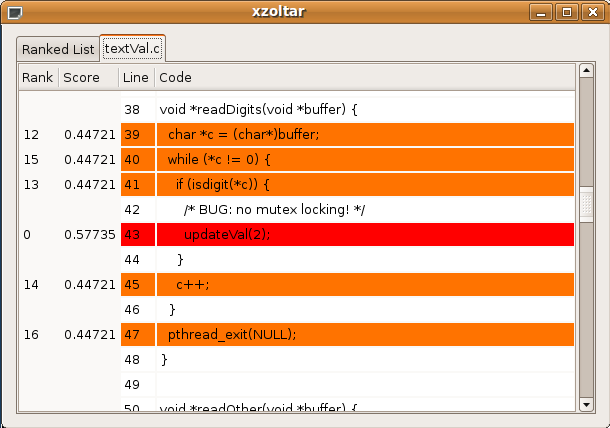
\includegraphics[scale=0.40]{sources/ganalyze_textVal.png} \\
		\end{tabular}
		\end{center}
		\caption{Visualization of SFL in the textVal source code.}
		\label{fig:ganalyzeTextVal}
	\end{figure}
	
	In Figure \ref{fig:ganalyzeTextVal} the \verb|xzoltar| tool shows the 
	highest ranking location in the code.
	It turns out that the call to \verb|updateVal| without locking the mutex
	correlates most with the failing test runs.
	Even without having been part of the implementation process,
	a person debugging this program could use this tool, get these results,
	and notice that another thread function does lock the mutex when calling the same function.
		
	It is important to realize that this tool will not explain why an error occurred.
	It statistically determines the most probable location a fault could reside.
	However, it gives a very useful starting point for inspecting the code.
	It can serve as a director in the debugging process,
	offering a list of source code locations to inspect.

	In some situations the gathered run-data becomes outdated.
	This happens when the test set is revised and a new test suite needs to
	be run starting with a clean sheet.
	Another possibility for outdated run-data is when the program
	is instrumented anew.
	This will invalidate the information in \verb|datafile.dat|.
	In these cases the datafile needs to be renamed or removed.
	After removal, the datafile is created again with the next test run.
	The instrumented program is able to detect if an existing datafile
	conflicts with the current instrumentation
	and will abort and give a message to that extend.
	Renaming the datafile could be used to save run-data for different
	test suites.
	The results of each suite can be examined at a later moment by 
	specifying the datafile as an argument to \verb|zoltar| (or \verb|xzoltar|):\\
	\verb|  # zoltar --datafile=/path/to/datafile.dat|\\

	This concludes the basic program analysis example.
	The next chapter will discuss the instrumentation for program spectra in more detail.
	Chapter \ref{c:AutomaticErrorDetection} will explain instrumentation of the program
	to enable automatic error detection.
	This is used to pinpoint the location for the second bug in the \verb|textVal| program.

	
	







% To analyze a program, its source code must be available.
% The program \emph{P} will be instrumented according to the needs and situation and will be transformed to \emph{P'}.
% Using the software package it is done in the following way.

% \begin{itemize}
  % \item{intermediate bytecode is generated\\
    % \verb| llvm-gcc -g -c program.c -o program.bc|}
  % \item{instrumentation is performed\\
    % \verb| instrument -spblock -memprotection -bypassmain program.bc > program.bc.p|}
  % \item{compile into native machine code\\
    % \verb| llvm-llc program.bc.p > program.s|}
  % \item{link with library and generate executable\\
    % \verb| gcc -linstrument program.s -o program|}
% \end{itemize}


	% Several optional instrumentation \emph{passes} are available.
	% These instrumentations can be categorized as follows.

	% \begin{itemize}
	  % \item{bypassing the main function}
	  % \item{instrumentation to generate program spectra}
	  % \item{instrumentation for program invariants}
	  % \item{memory protection}
	% \end{itemize}

	% There are some requirements for the input of the instrumentation.
	% \begin{itemize}
	  % \item{programs that are to be instrumented must contain a main function}
	  % \item{before instrumenting a program has to be pre-compiled to LLVM byte code}
	  % \item{pre-compilation should involve adding debug information (-g option)}
	% \end{itemize}

	% An important instrumentation pass, one that needs to be executed always,
	% is the pass that bypasses the \verb|main|
  
%---------------------------------------------------------------------------------
\chapter{Spectrum Generation}
\label{c:ProgramSpectrumGeneration}



A program spectrum is a set of counters for the execution of given program locations
(although SFL usually only considers hit spectra).
For example, if a function \verb|f| of a program is instrumented,
then during the execution of the program the counter associated with \verb|f| is incremented each time \verb|f| is called.
The available instrumentation passes for generation program spectra are given in Table \ref{t:programspectra}.
Every instrumentation should include the \verb|bypassmain| instrumentation pass 
for the analysis library to be able to handle the instrumented code.
In the next sections the different program spectra are discussed in more detail.


\begin{table}
  \begin{center}
  \begin{tabular}{l|l}
    name & description \\
	\hline
    -spbasicblock & instrument basic blocks \\
	-spfunction & instrument functions \\
	-spdefuse & instrument define-use pairs \\
  \end{tabular}
  \caption{instrumentation passes for generation of program spectra}
  \label{t:programspectra}
  \end{center}
\end{table}



\section{Basic Blocks}

	Basic blocks of code are defined as a sequence of statements with one entry point and one exit point,
	having no jump instructions contained within it.
	Basic blocks can be considered the basic unit of a program with respect to control flow.
	Whether a basic block is executed or not, or the number of times a certain basic block is executed, 
	can give useful information on the influence of this block on a failing execution of the program.
	
	In the basic block instrumentation pass, basic blocks are retrieved from the LLVM intermediate representation.
	It must be noted that the LLVM intermediate code sometimes contains additional basic blocks, 
	due to the generation of additional blocks which do not change the control flow.
	For example, a block is generated by default at the end of a function to contain the function return,
	although that function may consist of a single block of control flow with no branches.
	However, since the set of LLVM basic blocks is always a superset of the usual set of basic blocks,
	the resulting spectrum can be considered equally usable for further analysis.

	Performing basic block instrumentation is done using the \verb|-spbasicblock| option of the \verb|instrument| tool.
	For example,\\
	\verb|  # instrument -spbasicblock -bypassmain textVal.bc -o textVal.ibc|\\
	will instrument basic blocks and will perform the necessary bypass of the main function.

	

\section{Functions}

	The entry of every function in the program can be instrumented.
	Each time a function is called, the corresponding counter will be incremented.
	This can be useful in situations in which a project contains many small functions
	and a function containing the fault must be localized.
	This will not be as accurate as basic block instrumentation, 
	but the overhead will be limited, since there are far less functions
	in a program than there are basic blocks.
	
	Performing function instrumentation is done using the \verb|-spfunction| option of the \verb|instrument| tool.
	For example,\\
	\verb|  # instrument -spfunction -bypassmain textVal.bc -o textVal.ibc|\\
	will instrument every function and will perform the necessary bypass of the main function.
	It must be noted that the order of instrumentation passes is important in this case,
	since the new main function will be instrumented in the case that the \verb|bypassmain|
	instrumentation is performed before the \verb|spfunction| pass.
	This will result in a distorted source code context.
	The rule is that the \verb|bypassmain| is always last in the chain of instrumentation passes.


\section{Def-Use Pairs}

	A variable is defined once in its lifetime.
	This instance of a variable can be used at different locations of the program.
	The def-use spectrum contains a counter associated with each of these \emph{uses}.
	One variable can have multiple uses and therefor have multiple counters in the spectrum.
	Whenever, during the execution of the program, a variable is used, 
	the counter associated with that particular use is incremented.
	
	Performing def-use instrumentation is done using the \verb|-spdefuse| option of the \verb|instrument| tool.
	For example,\\
	\verb|  # instrument -spdefuse -bypassmain textVal.bc -o textVal.ibc|\\
	will instrument every use of declared variables and will perform the necessary bypass of the main function.
	
	Currently, the source code location of these uses are not reflected well in the generated context.
	The results when using this option are, for the time being, harder to interpret.

	
\section{Custom Program Spectra}

	The instrumentation of program points for generating program spectra is not limited to the discussed instrumentations.
	A custom pass can be created to obtain run time information of the program 
	suited to the needs of a specific analysis.
	The technical information needed for implementing custom instrumentation passes 
	is discussed in detail in Appendix \ref{c:WritingInstrumentationPasses}.
	
	
	

	% \begin{exercise}{Basic Block Instrumentation}
	% Compile the source code of RationalSort.c to LLVM byte code containing debug information using the LLVM gcc-frontend:\\
	% \verb|# llvm-gcc -emit-llvm -g -c RationalSort.c -o RationalSort.bc|\\
	% Then, instrument the byte code with basic block spectrum information gathering functionality.
	% Note that bypassing of main is required for instrumentation to have effect:\\
	% \verb|# instrument -spblock -bypassmain RationalSort.bc > RationalSort.ibc|
	% \end{exercise}
	  
	% \begin{exercise}{Inspect Instrumentation}
	% Convert the instrumented byte code back to C code:\\
	% \verb|# llc -march=c RationalSort.ibc -o RationalSort_i.c|\\
	% Inspect the code.
	% Notice that LLVM generates a large amount of extra code when translating LLVM byte code back to C.
	% Locate the \verb|_updateSpectrum| calls in the code.
	% These are the actual points in the program that are instrumented (at the beginning of each basic block).
	% Verify that there is no \verb|main| method and that the original \verb|main| method is replaced by \verb|_main_original|.
	% \end{exercise}

 
%---------------------------------------------------------------------------------
\chapter{Automatic Error Detection}
\label{c:AutomaticErrorDetection}


During the design phase of a program test oracles are usually available.
However, this is not the case during the operational stage of a program.
We do need some form of error detection for the SFL technique to work.
To facilitate debugging of a program in this stage we would like to have
a test oracle as in the design state, however this would require automatic
generation of invariants based on the program specifications, which is 
hard and currently not done in practice.
Also, the detailed program specifications needed to achieve this are usually
unavailable.

Secondly, some program faults cause a crash of the program,
or cause the program to hang at a certain point.
Next to that, determining correct execution is often more difficult than simply comparing outputs.
Examples of these programs are programs with buggy user interfaces,
continuous programs with sparse buffer overflow events, etcetera.
Implementing application-specific invariants to detect these bugs is an expensive task 
and very error-prone and often incomplete, as it is done manually.
Rather, we would like simple, generic program invariants,
which can be automatically trained to become application specific.
In combination with the fault localization techniques, 
this automatic error detection could ultimately evolve into
a fully automated fault localization,
given that a program is trained for normal behavior using the test oracle
during the design phase.


In the \verb|textVal| example (Section \ref{s:exampleProgram}), 
the first five test inputs result in an output which can easily be verified.
However, the sixth test input causes the program to hang.
No output is returned, so it can not be verified, 
although the behavior is such that we know that this run fails expected execution.
In normal cases, a \verb|^C| command will stop execution of the program,
but will update the spectrum data before shutting down to keep the important data of this failing run.
Because of the threaded nature of this program the program keeps blocking
and termination of the program is only possible with a kill signal.

To monitor programs for errors, the tool set is able to instrument programs to
automatically detect errors and stop the running program, while recording a failed run.
This is done by training certain program invariants and enabling screeners to trigger the fault.
Program invariants and fault screeners are discussed in the next sections.
Finally, the \verb|textVal| program is instrumented with an invariant type 
to demonstrate automatic error detection and to help find the second bug.


\section{Program Invariants}

	Program invariants are predicates that should hold throughout the execution of the program.
	For example, each loop in the program can hold an invariant which expresses the maximum number of iterations.
	During the training phase with expected behavior of the program, this maximum number is updated.
	During the testing phase, if the number of iterations exceeds the recorded value, 
	the program invariant is violated and an error is generated.

	The \verb|instrument| tool is able to instrument different types of invariants.
	A summary of these invariant types is given in Table \ref{t:programInvariants}.
	Each of these invariant types will be discussed in the next sections.

	\begin{table}
		\begin{center}
		\begin{tabular}{l|l}
			name & description \\
			\hline
			-invstore         & instrument store invariants \\
			-invload          & instrument load invariants \\
			-invlooploop      & instrument loop counter invariants \\
			-invfunctiontimer & instrument function timing invariants \\
		\end{tabular}
		\caption{instrumentation passes for program invariants}
		\label{t:programInvariants}
		\end{center}
	\end{table}


\subsection{Stores}

		Every time a value is written to memory this is monitored when the program is instrumented
		with the \verb|store| invariant type.
		If an unexpected value is stored (e.g., a value outside an array bound) according to the training phase,
		an error is generated.
	
		Performing instrumentation for the \verb|store| invariant type is done using the 
		\verb|-invstore| option of the \verb|instrument| tool.
		For example,\\
		\verb|  # instrument -invstore -bypassmain textVal.bc -o textVal.ibc|\\
		will instrument stores and will perform the necessary bypass of the main function.

\subsection{Loads}

		Every time a value is loaded from memory this is monitored when the program is instrumented
		with the \verb|load| invariant type.
		If an unexpected value is loaded (e.g., a NULL pointer), according to the training phase,
		an error is generated.	

		Performing instrumentation for the \verb|load| invariant type is done using the 
		\verb|-invload| option of the \verb|instrument| tool.
		For example,\\
		\verb|  # instrument -invload -bypassmain textVal.bc -o textVal.ibc|\\
		will instrument loads and will perform the necessary bypass of the main function.


\subsection{Loop Counters}

		The \verb|instrument| tool is able to get information of execution loops
		existing in the program
		and instrument it to count the number of consecutive iterations of each loop.
		Most of the time, these loops will have a limited number of iterations during execution.
		The \emph{normal} number of iterations can be trained when the program is run on input
		resulting in expected behavior.
		This invariant type is very useful for situations where unexpected endless loops occur
		causing the program to stop functioning.

		Performing instrumentation for the \verb|loop counter| invariant type is done using the 
		\verb|-invloopcount| option of the \verb|instrument| tool.
		For example,\\
		\verb|  # instrument -invloopcount -bypassmain textVal.bc -o textVal.ibc|\\
		will instrument the counting of loop iterations and will perform the necessary bypass of the main function.

	
\subsection{Function Timing}

		The instrumentation of the program supports timed invariants as well.
		The function timing invariant monitors the time that is spent within a function.
		A timer with a 1 ms interval signals an increment of every function which is \emph{active},
		i.e., which is still in the process of being executed.
		At the start of a function execution the counter is set to zero.
		During the training phase, every millisecond a program remains in a function this is recorded.
		If, during testing, the program remains in that function for longer than it should,
		an error is generated.

		Performing instrumentation for the \verb|function timing| invariant type is done using the 
		\verb|-invfunctiontimer| option of the \verb|instrument| tool.
		For example,\\
		\verb|  # instrument -invfunctiontimer -bypassmain \ | \\
		\verb|  > textVal.bc -o textVal.ibc|\\
		will instrument functions for timing and will perform the necessary bypass of the main function.


\subsection{Custom Invariant Instrumentation}

		As with the program spectra, 
		custom instrumentation passes can be created for instrumenting the program for other invariants.
		The technical information needed for implementing custom instrumentation passes 
		is discussed in detail in Appendix \ref{c:WritingInstrumentationPasses}.

		
	
\section{Fault Screeners}

	Fault screeners are used to train and monitor each variable that is instrumented as invariant.
	Different types of fault screeners exist, 
	determining the possible values an instrumented variable assumes.
	The invariant of the variable is that the variable remains within the trained set of values.
	The currently supported screeners are a range screener and a bit mask screener.
	These are discussed in the following sections.

\subsection{Range}

		When a range screener is enabled for an invariant, 
		the minimum and maximum values an instrumented variable obtains during training is recorded.
		If, during testing, the variable suddenly assumes a value outside of this range,
		an error is generated.

\subsection{Bit Mask}

		A bit mask screener monitors the actual bits of a variable.
		Bits that are changed during execution are marked in the training phase.
		If, in the testing phase, an unexpected bit is changed, an error is generated.

%\subsection{Bloom Filter}

%\section{Training and Testing}


\section{Automatic Error Detection in Practice}
	
	To demonstrate automatic error detection we will try to locate the second bug in the \verb|textVal|
	program.
	As mentioned previously, the sixth test input will cause the program to hang.
	This erratic behavior can be caught by instrumenting the program to generate an error if
	the program remains within a function for too long.
	The tool set offers the \verb|function timing| instrumentation for this purpose.
	The \verb|textVal| program will now be instrumented using the following commands.\\
	\verb|  # llvm-gcc -g -emit-llvm -c textVal.c -o textVal.bc| \\
	\verb|  # instrument -f -invfunctiontimer -spbasicblock \ | \\
	\verb|  > -bypassmain textVal.bc -o textVal.ibc| \\
	\verb|  # llc -f textVal.ibc -o textVal.s| \\
	\verb|  # gcc textVal.s -lpthread -linstrument -o textVal| \\

	The resulting executable must now be trained with normal behavior
	(i.e., input test data for which the program test is known to pass)
	to be able to detect abnormal behavior.
	To do this we simply execute the program with test inputs which not cause the program to hang.
	The instrumented program is in training mode by default.
	In other words we may use the same sequence of tests as before.
	But before that, the existing data file must be removed, 
	since it is not compatible with the newly instrumented version.
	The instrumented program will complain about this if it does find an existing incompatible data file.\\
	\verb|  # rm datafile.dat|\\
	\verb|  # ./textVal < test1.in|\\
	\verb|  # ./textVal < test2.in|\\
	\verb|  # ./textVal < test3.in|\\
	\verb|  # ./textVal < test4.in|\\
	\verb|  # ./textVal < test5.in|\\
	
	At this point the invariant is trained with expected values.
	This can be viewed and edited by the \verb|zoltar| tool.
	To do this, we start the \verb|zoltar| tool as discussed previously.
	In the main menu we select \verb|Invariants| to view all instrumented invariant types.
	We select the \verb|Function Timer| invariant and we will be presented with some options
	for modifying the invariant training values.
	We select \verb|Edit invariants| to view the trained values.
	
	With the \emph{left} and \emph{right} keys the trained values corresponding to the 
	\verb|range| screener and \emph|bit mask| screener can be viewed and edited.
	Also, the screeners can be enabled and disabled to the wishes of the user.
	This can be useful in cases in which you know that a value can assume any value,
	although this is not trained, e.g., random values or pointers.
	
	The trained values are very strict.
	In this case, the time spent in a function is related to the size of the input,
	which may vary.
	To be able to support a wider range of inputs, 
	we can stretch these values, introducing a safe margin.
	Only if an unexpected large amount of time is spent in a function we want an error to be generated.
	To return to the previous screen we press the \emph{backspace} key.
	We can now select the \verb|stretch 100% (MAX only)| option to double the range of the 
	valid number of milliseconds a function may be executed.
	After this is done, the new values are shown.
	To be sure, we will repeat this one more time, to get a very reasonable range of execution time.
	The resulting values are shown in the screenshot of the \verb|zoltar| program in 
	Figure \ref{fig:analyzeInv}.
	
	\begin{figure}[h!]
		\begin{center}
		\begin{tabular}{c}
			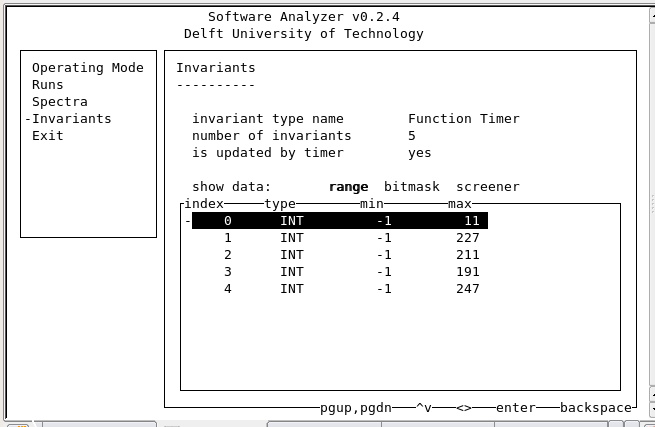
\includegraphics[scale=0.40]{sources/analyze_inv.png} \\
		\end{tabular}
		\end{center}
		\caption{Invariant training of the textVal program.}
		\label{fig:analyzeInv}
	\end{figure}

	Next, the program has to be set to testing mode in order to be able to detect and react upon an 
	error caused by an invariant violation.
	To do this, we press \emph{backspace} a number of times until the main menu is active.
	In the summary the operating mode is shown to be set to \verb|training|.
	We select \verb|Operating Mode| from the menu and select \verb|testing| to configure the program
	for automatic error detection.
	When this is done, we press the '\emph{q}' key or go to the main menu and select \emph{exit}.
	
	At this moment the instrumented program is trained and ready to handle invariant violations.
	Now we can test the sixth test input using the following command.\\
	\verb|  # ./textVal < test6.in|\\
	During the execution a range invariant has been violated and an error is generated accordingly.
	If the \verb|zoltar| tool is started again, the status of all runs can be examined.
	Select \verb|Runs| from the main menu and notice that the sixth run has automatically been 
	given the \emph{failed} status, because during that run an error occurred.
	Exit the \verb|zoltar| tool and start \verb|xzoltar| to perform SFL analysis
	and give visual feedback in the source code.
	
	\begin{figure}[h!]
		\begin{center}
		\begin{tabular}{c}
			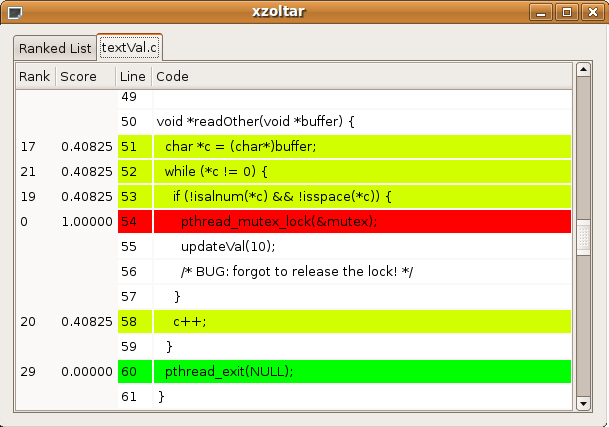
\includegraphics[scale=0.40]{sources/ganalyze_bug2.png} \\
		\end{tabular}
		\end{center}
		\caption{Visualization of the SFL result showing the location of the second bug.}
		\label{fig:ganalyzeBug2}
	\end{figure}

	The relevant piece of code according to the SFL results is given in Figure \ref{fig:ganalyzeBug2}.
	It shows that the basic block starting at line 54 in the code corresponds most with the run
	which resulted in an error.
	This is indeed within the function of the third thread scanning for non-alphanumeric characters.
	The actual block is the part which does lock the mutex, but does not unlock it.
	
	Using this tool set we are able to locate faults for various types of faults,
	including the rather difficult faults in which lines of code are missing, 
	as demonstrated in this tutorial.
	No knowledge about the software under test is required.
	The output of the tool can help software developers to investigate their code more efficiently,
	by being lead to the most probable locations at which the fault could be.
	

 
%---------------------------------------------------------------------------------
\chapter{Analyzing Large Programs}
\label{c:AnalyzingLargePrograms}

%\emph{This chapter will discuss the instrumentation and analysis of
%large programs, consisting of many source files. 
%Partial instrumentation is supported by the Zoltar toolset.}

Realistically sized programs usually consist
of 100.000s of LOC and hundreds of files.
Instrumenting all of it on the basic block level
could result in an undesirable slowdown,
a large amount of runtime data,
and could even be impossible to instrument
(before instrumentation every file has to be
linked into one intermediate LLVM bytecode file).

To overcome this problem some instrumentation
and analysis strategies can be implemented
using partial instrumentation.

If the speed of the instrumented program is
compromised or the generated datafile is too
large, one can opt to instrument on function
level initially.
This will reduce the size of the datafile
and will result in a fault localization that
is less detailed.
Using these results, however, one can then
select the top ranking files, which are most
likely to contain the fault, for a more
fine-grained instrumentation, for example
on the basic block level.
Less basic blocks are instrumented,
compared to instrumenting the complete program,
resulting in a more manageable datafile and better
performance of the instrumented executable.

	\begin{figure}[h!]
		\begin{center}
		\begin{tabular}{c}
			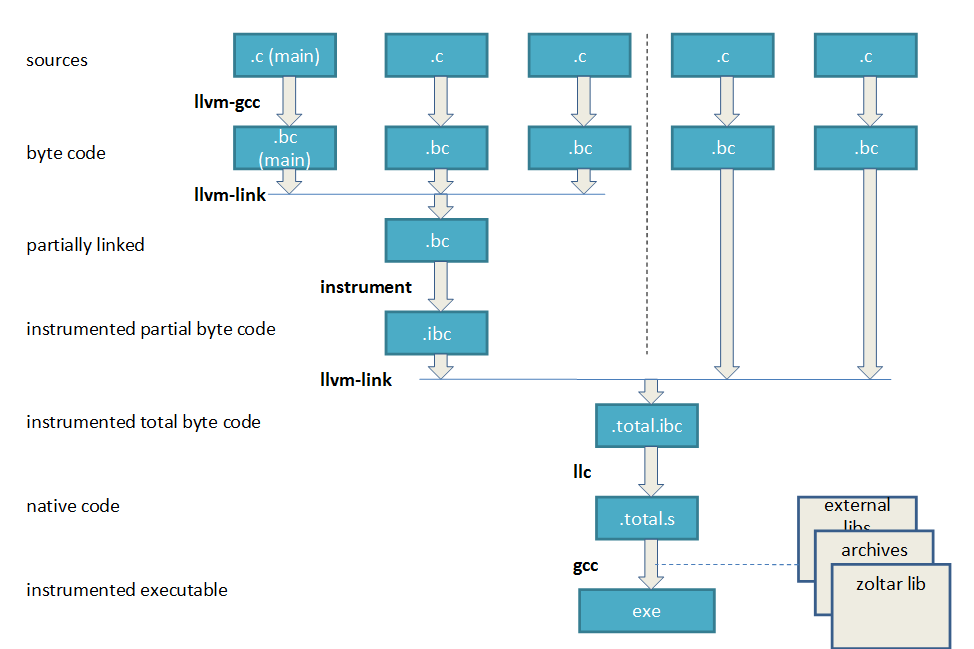
\includegraphics[scale=0.30]{sources/partial_instrumentation.png} \\
		\end{tabular}
		\end{center}
		\caption{Partial instrumentation.}
		\label{fig:partialInstrumentation}
	\end{figure}

The general instrumentation procedure,
supporting partial instrumentation,
is illustrated in Figure \ref{fig:partialInstrumentation}.
It shows that all source files are first
converted to LLVM bytecode.
A selection of these bytecode files,
including the file with the main function,
are then linked together and instrumented.
In the next step, the resulting instrumented bytecode
is linked with the remaining bytecode
that was not instrumented.
Finally, native code is generated and all is
linked with other archives of the program,
external libraries and the Zoltar library.
Note that having internal libraries or archives
can reduce the total size of the linked bytecode
file just before converting to native code.
LLVM could have problems if this were too large.
However, if some of these libraries are to be
instrumented as well, their source files should
be linked to the main source file before instrumenting,
as instrumentation of a program can not be done
on various source files separately.




%---------------------------------------------------------------------------------
\chapter{Batch Execution}
\label{c:BatchExecution}

%\emph{This chapter will contain information on the support for
%command line input and output to enable batch execution for large 
%test sets.}

In realistic cases, tests are usually performed in an automated way,
using a large test suite.
The Zoltar toolset offers command line input, 
next to the interactive user interface, 
to be able to process a large amount of tests using a script.

During the runtime data gathering process, 
the script can compare the output with an expected output,
or use some other means of error detection.
The resulting passing or failing of a run
can be recorded in a separate file 
(writing a 1 for a passed run and a 0 for a failed run).
Additionally, if instrumented and trained for 
automatic error detection,
the runs in which invariants are compromised
are marked as failed within the datafile.

The external \verb|passfail| file can be given as input
to the \verb|zoltar| and \verb|xzoltar| tools,
which combine the information on failing runs from
the passfail file and the datafile.
A run which is marked as failed in either file is
considered failed in the analysis.

The \verb|zoltar| tool is able to immediately return 
SFL results when given the following command line options:\\
\verb|  # zoltar --passfailfile=passfail.out --sfl=ochiai|\\
This will return the complete listing of the ranked 
fault locations, using external passfail information in
the \verb|passfail.out| file.
This list can be in the order of thousands, 
for example, if a realistically sized program
is instrumented on the basic block level.
This list can be cut off using an additional argument
on the command line:\\
\verb|  # zoltar --passfailfile=passfail.out --sfl=ochiai -n10|\\
This will result in a ranked list of program locations
limited to ten results, given as output in the console (on \verb|stdout|).
This feature can be used for intermediate results in 
automated testing of a program using a large test suite.
With information of more test runs this intermediate result
will typically be improved.

The index of the spectrum on which the SFL technique is applied,
can be set using the \verb|-i| command line argument.
For example, if a program is instrumented to generate 
spectra for basic blocks and for def-use pairs,\\
\verb|  # zoltar --sfl=ochiai -n10 -i1|\\
will immediately return the first ten SFL results
of the ranked list of def-use locations,
given that the basic block spectrum has index 0
and the def-use spectrum has index 1.
These indices depend on the order in which the instrumentation passes
are given in the instrumentation command (see Section \ref{s:instrumentation}).

Using an external passfail file one can imagine scripts that
will execute a large number of tests, taking days or weeks to complete, 
while producing intermediate results for early analysis.
The support of an external passfail file and the command line functionality 
make the Zoltar toolset flexible and fit for many test situations.


%---------------------------------------------------------------------------------
%---------------------------------------------------------------------------------
\appendix

%---------------------------------------------------------------------------------
% \chapter{Spectrum-based Fault Localization}
% \label{c:SFL}

% \input{tech_sfl}

%---------------------------------------------------------------------------------
\chapter{Writing Instrumentation Passes}
\label{c:WritingInstrumentationPasses}


To be able to write custom instrumentation passes,
one must have some knowledge of the LLVM intermediate
representation and of the LLVM API.
The documentation of LLVM can be found at
\verb|http://llvm.org|.
Most interesting in this context is the document that
handles writing an LLVM pass, which is located at
\verb|http://llvm.cs.uiuc.edu/docs/WritingAnLLVMPass.html|.
Keep in mind that the LLVM version supported by
the Zoltar toolset is version 2.4, 
meaning that the correct API documentation should be consulted.

The instrumentation passes are located in the 
\verb|/lib/passes/| directory within the Zoltar 
source tree.
Each pass is in fact an optimization pass
in the concept of LLVM.
Each pass is a subclass of a \verb|ModulePass|,
a \verb|FunctionPass| or a \verb|LoopPass|,
but typically a \verb|ModulePass| should be
used as the superclass of an instrumentation pass.
The function that will be called during the instrumentation
is \verb|runOnModule|, 
which will contain the code to modify the LLVM bytecode.
Within a ModulePass we have the ability to
iterate through all functions and we can access
all variables.
This will be explained in the following sections.

When changing parts of the intermediate code,
care must be taken not to change the workings
of the original program, for example,
by inserting a new branch.

To be able to relate the instrumentation points to the
lines of code in the source file, debug information must
be extracted as well.
How this is done is shown in the example instrumentation
pass in the last section of this appendix.




\section{Inserting Instrumentation Code}

To instrument a location within the program,
the exact location must first be found.
For example, when instrumenting program points to
generate a spectrum on the function level,
we must navigate to the beginning of each function.
Then, conform the LLVM intermediate representation rules,
new instructions can be added after the initial instructions
for allocating memory.

We can use the following constructs to iterate
through functions, basic blocks and instructions:

\begin{lstlisting} [numbers=none]
/* in the runOnModule function: */
  // M is the Module, argument of runOnModule
  // Loop through all functions within module
  for (Module::iterator F = M.begin(), ME = M.end(); 
       F != ME; ++F) {
    // Loop through all basic blocks within function
    for (Function::iterator B = F->begin(), FE = F->end(); 
         B != FE; ++B) {
      // Loop through all instructions within basic block
      for (BasicBlock::iterator I = B->begin(), BE = B->end(); 
        I != BE; I++) {
        // process Instruction *I
      }
    }
  }
\end{lstlisting}

When the correct location is found,
instructions can be added to call a library function
to indicate that this program point is being executed,
or that a certain variable has been changed.

The LLVM framework provides the means to analyze the
execution tree and, for example, can provide a way to
iterate through all existing loops within a function.
To achieve this, the function
\verb|getAnalysisUsage| should be overridden in the pass
and should contain a \emph{LoopInfo} analysis requirement.
As a result, the LoopInfo pass (standard LLVM pass) is run 
in advance, so that information of loops within the program
is available.

\begin{lstlisting} [numbers=none]
// override getAnalysisUsage
void getAnalysisUsage(AnalysisUsage &AU) const {
  // indicate that the pass does not change the LLVM program
  AU.setPreservesAll();
  // makes sure that the LoopInfo pass is run in advance
  AU.addRequired<LoopInfo>();
}

/* in the runOnModule function: */
    // get loop info analysis from LLVM
    LoopInfo &LI = getAnalysis<LoopInfo>(*F);

    // process all loops in function
    for (LoopInfo::iterator L = LI.begin(), LE = LI.end(); 
         L != LE; ++L) {
      // process Loop *L
    }
\end{lstlisting}

This is used in creating the \verb|loopcount| invariant pass.


\subsection{Program Spectrum}

A call to the library function \verb|_updateSpectrum| is inserted
in the LLVM intermediate representation to generate spectrum
information on that point in the program.
This program point can mark the beginning of a function or the
basic block, it can be located in front a certain type of instruction
or it can be any other type of program point.
What is relevant here is that there is a spectrum item
that refers to the execution of a single point in the program.

The \verb|_updateSpectrum| function has the following prototype.
\begin{lstlisting} [numbers=none]
void _updateSpectrum(unsigned int spectrumIndex, 
                     unsigned int componentIndex);
\end{lstlisting}

Multiple spectra can be instrumented within the same program.
These are distinguished by the spectrum index.
Each spectrum contains a number of program points that are instrumented.
For example, if both the function spectrum and the basic block spectrum 
are instrumented, one has index 0 and the other will have index 1.
The function spectrum contains a number of instrumented program points
equal to the number of functions in the instrumented program.
Each instrumented point has its own index to be able to correctly update
the spectrum during execution.

The Zoltar library contains an \verb|IndexManager| to keep track of the
indices of the spectra and invariant types.
The index of the current spectrum should be requested before instrumenting
the LLVM code, i.e., at the start of the \verb|runOnModule| function.
The index of the current program point (componentIndex) is simply a counter
that starts at 0 and is incremented with each inserted call to the
\verb|_updateSpectrum| library function.
The relevant code to insert spectrum points in the LLVM bytecode is
given in the following code.
\begin{lstlisting} [numbers=none]
// include the index manager
#include "indexManager.h"

/* in the runOnModule function: */
  // Add library function prototype
  Constant *SpFn = M.getOrInsertFunction("_updateSpectrum", 
                          Type::VoidTy, 
                          Type::Int32Ty,  // spectrum index
                          Type::Int32Ty,  // component index
                          NULL);

  // get the correct index of the current spectrum
  unsigned spectrumIndex = IndexManager::getSpectrumIndex();

  // initialize the component index counter
  unsigned nComponents = 0;

/* in the runOnModule function, at an insertion point: */
    // create the arguments to the library function
    std::vector<Value*> Args(2);
    Args[0] = ConstantInt::get(Type::Int32Ty, spectrumIndex);
    Args[1] = ConstantInt::get(Type::Int32Ty, nComponents++);
    
    // insert a call to the _updateSpectrum function
    //   just before the LLVM instruction I
    CallInst::Create(SpFn, Args.begin(), Args.end(), "", I);
\end{lstlisting}

At the end of the spectrum instrumentation pass, 
the currently created pass should be registered in the initial
part of the resulting program.
This is required to be able to allocate and initialize 
a sufficient amount of memory.
This is done by means of the \verb|addSpectrumRegistration|
function, which has the following prototype.
\begin{lstlisting} [numbers=none]
void addSpectrumRegistration(Module &M,
                             int spectrumIndex, 
                             int nComponents, 
                             const std::string &SpectrumName);
\end{lstlisting}

The Module (which is an argument to the runOnModule function) 
is given as argument to the function.
This is required to insert an initialization function that 
processes all registered instrumentation passes.
The \verb|spectrumIndex| argument is the index of the current
spectrum, which was retrieved by the \emph{IndexManager}.
The \verb|nComponents| argument is the number of instrumented
program points during this pass, i.e., the final value of the
program point counter.
The \verb|SpectrumName| argument should be a short (no more than 16 characters)
informative description of the instrumentation.
This will be used in the analysis tools to represent the spectrum.
For example, the basic block spectrum instrumentation pass
creates a spectrum with the name \verb|Basic_Blocks|.


\subsection{Invariant Type}
\label{s:appendixInvariantType}

Multiple library functions exist for instrumenting invariants.
These are based on the type of the variable that is instrumented.
We distinguish the following invariant change library functions.
\begin{lstlisting} [numbers=none]
void _handleInvariantChangeDouble(unsigned int invTypeIndex, 
                                  unsigned int invIndex, 
                                  double val);
void _handleInvariantChangeInt(unsigned int invTypeIndex, 
                               unsigned int invIndex, 
                               int val);
void _handleInvariantChangeUInt(unsigned int invTypeIndex, 
                                unsigned int invIndex, 
                                unsigned int val);
void _handleInvariantChangePtr(unsigned int invTypeIndex, 
                               unsigned int invIndex, 
                               void *val);
void _handleInvariantIncrement(unsigned int invTypeIndex, 
                               unsigned int invIndex);
\end{lstlisting}
All these functions signify a change of an instrumented variable,
corresponding to the invariant with index \texttt{invIndex} of the
invariant type with index \verb|invTypeIndex|.
The four types that are distinguished are \texttt{double}, 
\texttt{int}, \texttt{unsigned int} and the \texttt{void pointer} type.
To efficiently support an invariant based on a counter,
the library also contains an increment library function, 
which simply adds 1 to a certain variable corresponding to the given 
invariant index.

Similar to the code of the spectrum instrumentation,
the following pieces of code is used to insert invariant
instrumentation.
It checks the type of the variable,
extracts the appropriate information, type casts correctly,
and calls the library function.
\begin{lstlisting} [numbers=none]
// include the index manager
#include "indexManager.h"

/* in the runOnModule function: */
  // Add library function prototypes
  Constant *handleDoubleFn = M.getOrInsertFunction(
    "_handleInvariantChangeDouble", 
    Type::VoidTy,   // returns void
    Type::Int32Ty,  // invTypeIndex
    Type::Int32Ty,  // invIndex
    Type::DoubleTy, // val
    NULL);
  Constant *handleIntegerFn = M.getOrInsertFunction(
    "_handleInvariantChangeInt", 
    Type::VoidTy,   // returns void
    Type::Int32Ty,  // invTypeIndex
    Type::Int32Ty,  // invIndex
    Type::Int32Ty,  // val
    NULL);
  Constant *handlePointerFn = M.getOrInsertFunction(
    "_handleInvariantChangePtr", 
    Type::VoidTy,   // returns void
    Type::Int32Ty,  // invTypeIndex
    Type::Int32Ty,  // invIndex
    PointerType::getUnqual(Type::Int32Ty),  // val
    NULL);
  Constant *handleUintFn = M.getOrInsertFunction(
    "_handleInvariantChangeUInt", 
    Type::VoidTy,   // returns void
    Type::Int32Ty,  // invTypeIndex
    Type::Int32Ty,  // invIndex
    Type::Int32Ty,  // val
    NULL);

  // get the correct index of the current invariant type
  unsigned int invariantTypeIndex = 
    IndexManager::getInvariantTypeIndex();

  // initialize the counter for the invariant index
  unsigned int nInvariants = 0;

/* in the runOnModule function, at an insertion point: */
    // Value Val is the value to instrument
    const Type *InstType = Val->getType();
    std::vector<Value*> Args(3);
    if(InstType->isInteger()) {
      // create the arguments to the library function
      Args[0] = ConstantInt::get(Type::Int32Ty, 
                                 invariantTypeIndex);
      Args[1] = ConstantInt::get(Type::Int32Ty, 
                                 nInvariants++);
      // insert a cast to int instruction before instruction I,
      //   the resulting value is passed to the library call
      Args[2] = CastInst::createIntegerCast(Val, 
                                            Type::Int32Ty, 
                                            true, 
                                            "inv.cast", 
                                            I);

      // insert call to the _handleInvariantChangeInt function
      //   just before the LLVM instruction I
      CallInst::Create(handleIntegerFn, 
                       Args.begin(), 
                       Args.end(), 
                       "", 
                       I);
    }
\end{lstlisting}

As is the case with spectrum instrumentation,
at the end of the invariant instrumentation pass 
the currently created pass should be registered in the initial
part of the resulting program.
This is done by calling the library function \texttt{addInvariantTypeRegistration}, 
which has the following prototype.
\begin{lstlisting} [numbers=none]
void addInvariantTypeRegistration(
  Module &M,
  int invariantTypeIndex, 
  int nInvariants, 
  const std::string &invariantTypeName, 
  int isTimerUpdated);
\end{lstlisting}
The arguments are the same as for the spectrum registration function,
except for the last argument.
This indicates if the invariant is based on a timer update.
If this is the case, the value of the invariant variable 
is not changed due to the value of a variable of the program
during execution.
Rather, it is incremented based on a timer interrupt each millisecond.

The timer will increment only if the current value is non-negative.
The instrumentation is responsible for resetting the value,
using the \texttt{\_handleInvariantChangeUInt} library function, 
if the instrumented point in the code is executed.
For example, to implement a function timer, 
the invariant variable can be set to 0 at the beginning of a function
and should be set to -1 at every endpoint of the function
to indicate that the value should not be incremented anymore.
This will result in a measurement of execution time of a function.
When this invariant is trained, an abnormal long execution of the function,
e.g., an endless loop, can be detected.



\section{A Practical Example}

An example instrumentation pass gives more insight of the 
way to navigate and process LLVM bytecode.
The basic block spectrum instrumentation pass included in
the Zoltar library is used as an example in this section.
The pass will be explained step by step.
Included in this example is the way in which debug information
is extracted to generate context information of the source file.

Before writing the actual pass, the necessary headers need to
be included. 
Among these headers are many LLVM headers, mainly for processing LLVM
bytecode.
Next to that we can include standard headers, e.g., \texttt{<fstream>}
for writing to files or to print messages to the console while 
instrumentation is in progress.
Finally, we need to include \texttt{indexManager.h} for retrieving the
correct index for the spectrum, 
\texttt{contextManager.h} which handles the generation of the context file,
and \texttt{registration.h} to register the instrumentation to the program.

\begin{lstlisting} [numbers=none]
#include "llvm/Constants.h"
#include "llvm/DerivedTypes.h"
#include "llvm/Instructions.h"
#include "llvm/Module.h"
#include "llvm/Pass.h"
#include "llvm/Support/Compiler.h"
#include "llvm/Support/Streams.h"
#include "llvm/Transforms/Instrumentation.h"
#include "llvm/ValueSymbolTable.h"
#include "llvm/Value.h"
#include "llvm/Support/CallSite.h"
#include "llvm/IntrinsicInst.h"
#include "llvm/Analysis/ValueTracking.h"
#include "llvm/Support/CFG.h"
#include "llvm/Target/TargetData.h"
#include "llvm/Analysis/LoopInfo.h"
#include <time.h>
#include <fstream>

#include "indexManager.h"
#include "contextManager.h"
#include "registration.h"
\end{lstlisting}

Next, we set the namespace and define the class of the instrumentation pass.
We call it \texttt{SPBasicBlockInstrumenter} and derive it from \texttt{ModulePass}.
The \texttt{runOnModule} function needs to be overridden.
The \texttt{char ID} is required for every LLVM pass and is used
for the actual registration of the pass in the instrumenter tool.

\begin{lstlisting} [numbers=none]
using namespace llvm;
using std::ofstream;

namespace {
  class SpBasicBlockInstrumenter : public ModulePass {
    bool runOnModule(Module &M);
  public:
    static char ID;
    SpBasicBlockInstrumenter() : ModulePass((intptr_t)&ID) {}
  };
}
\end{lstlisting}

The following lines sets the static \verb|ID| to 0 (this value should be set for all passes)
and the pass is registered to the \texttt{instrument} tool, 
using a static \texttt{RegisterPass} object.
The latter requires two arguments.
First is the name of the pass,
the second is a description of the pass.
This information will appear in the complete listing of passes
(LLVM optimization passes and Zoltar instrumentation passes)
when passing the \verb|--help| option to the \texttt{instrument} tool.
The name of the pass will be used as parameter to the
\verb|instrument| tool to run this instrumentation.
In this case, the \texttt{-spbasicblock} will instrument
basic blocks of the given program.

\begin{lstlisting} [numbers=none]
char SpBasicBlockInstrumenter::ID = 0;
static RegisterPass<SpBasicBlockInstrumenter>
  RPspblock("spbasicblock", 
            "Insert instrumentation for block hit spectrum");
\end{lstlisting}

Next begins the important \texttt{runOnModule} function.
At the start of the function, a notification is given on \texttt{stderr}.
The Module is checked for the main entry function.
If no main is present, the instrumentation is not possible and 
is aborted.

\begin{lstlisting} [numbers=none]
bool SpBasicBlockInstrumenter::runOnModule(Module &M) {

  cerr << "instrument: --- Basic Block Spectrum ---\n";

  Function *Main = M.getFunction("main");
  if (Main == 0) {
    cerr << "WARNING: cannot insert block instrumentation"
         << " into a module with no main function!\n";
    return false;  // No main, no instrumentation!
  }
\end{lstlisting}

The prototype of the \texttt{\_updateSpectrum} function needs to be 
inserted in the module and a reference is saved.
If it already exists (because of a previously executed instrumentation pass)
the reference to that function call is retrieved.
This reference is used later on to notify the library that the instrumented
point is executed.

\begin{lstlisting} [numbers=none]
  // Add library function prototype
  Constant *SpFn = M.getOrInsertFunction("_updateSpectrum", 
                          Type::VoidTy, 
                          Type::Int32Ty,  // spectrum index
                          Type::Int32Ty,  // component index
                          NULL);
\end{lstlisting}

In the following lines, the index of this spectrum is retrieved from 
the index manager, 
and the component counter is defined and initialized.

\begin{lstlisting} [numbers=none]
  unsigned spectrumIndex = IndexManager::getSpectrumIndex();
  unsigned nComponents = 0;
\end{lstlisting}

Next, every function in the module is visited and every basic block within
that function is visited.
Each of these basic blocks will be instrumented. 
While iterating through the functions, 
the functions which are only a declaration of a function are skipped, 
as they will not contain basic blocks.
Also take note of the register function, which will be called at the end of the instrumentation,
adds a function to the module for initializing the instrumentation data.
This function, (\texttt{\_registerAll}), should not be instrumented during the
instrumentation pass.
The current function is skipped if it has that specific name.
Each basic block is skipped if it is dead (if it is not the first basic block
of the function and it has no predecessors).

\begin{lstlisting} [numbers=none]
 // Loop through all functions within module
  for (Module::iterator F = M.begin(), ME = M.end(); 
       F != ME; ++F) {
    // skip function declarations
    if(F->isDeclaration()) 
      continue;

    // skip the _registerAll function
    if(F->getName()=="_registerAll")
      continue;

    // Loop through all basic blocks within function
    for (Function::iterator B = F->begin(), FE = F->end(); 
         B != FE; ++B) {
      //skip dead blocks
      BasicBlock *bb = B;
      if (B!=F->begin() && (pred_begin(bb)==pred_end(bb))) {
        continue; //skip dead blocks
      }
\end{lstlisting}

At this point we have a new basic block which needs to be instrumented.
To do this we iterate through all instructions within the 
basic block until we find the first debug stoppoint.
We know that at least one debug stoppoint will exist
in a basic block.
This is used by a debugger tool like \texttt{dbg} to step through the
execution of the program.
If a debug stoppoint LLVM instruction is found (\texttt{DbgStopPointInst}),
debug information of this program point can be extracted.
The file, path and line number are extracted from this instruction.
The name is irrelevant in this case, since a name for a basic block 
does not exist. We will use "-" for the name by default.

The ContextManager is responsible for creating the context file.
The information for each instrumented point is gathered by calling
the \texttt{addSpectrumContext} or \texttt{addInvariantContext} 
function while instrumenting a program point.
In this case we call \texttt{addSpectrumContext} and we give the
index of the spectrum and of the current program point (component), 
and all known information of the source location corresponding to
the current instrumented program point.


\begin{lstlisting} [numbers=none]
      // Loop through all instructions within basic block
      for (BasicBlock::iterator I = B->begin(), BE = B->end(); 
           I != BE; I++) {

        if(isa<DbgStopPointInst>(*I)) {
          DbgStopPointInst &DSPI = cast<DbgStopPointInst>(*I);
          std::string file, dir, name="-";
          llvm::GetConstantStringInfo(DSPI.getDirectory(), 
                                      dir);
          llvm::GetConstantStringInfo(DSPI.getFileName(), 
                                      file);
          int line = DSPI.getLine();

          // add source context of invariant to context file
          ContextManager::addSpectrumContext(
            spectrumIndex,     // spectrumIndex
            nComponents,       // componentIndex
            dir,               // path
            file,              // file
            line,              // line
            name);             // name
\end{lstlisting}

At this point we will do the actual instrumentation,
i.e., add a call to the \texttt{\_updateSpectrum} library function
at the beginning of the basic block.
Since the library function contains two arguments, 
we have to create a vector of LLVM Value objects and
fill them with the correct information of the spectrum index and
the index of the current component.
The component index is then incremented for the next basic block.
A call to the library function is inserted into the LLVM bytecode
just before the debug stoppoint,
which results in a spectrum update every time this basic block
is executed.
After inserting the call, the iteration through the basic block
can be aborted and the next basic block of the current function
is processed.
The same is done for all functions within the module.

\begin{lstlisting} [numbers=none]
          // add call to lib function
          std::vector<Value*> Args(2);
          Args[0] = ConstantInt::get(Type::Int32Ty, 
                                     spectrumIndex);
          Args[1] = ConstantInt::get(Type::Int32Ty, 
                                     nComponents++);
          
          CallInst::Create(SpFn, 
                           Args.begin(),  
                           Args.end(), 
                           "", 
                           I);

          break;
        }
      }
    }
  }
\end{lstlisting}

After all basic blocks are instrumented,
the spectrum needs to be registered using the
\verb|addSpectrumRegistration| function.
This will result in initialization of the spectrum data at 
the start of the instrumented program.
The function requires as arguments the module, the spectrum index, 
the total number of instrumented points of this instrumentation pass,
and the name of the instrumentation pass.
This name should not be too large and preferably contain no spaces,
to be correctly handled by the tools.

Finally, a summary message is printed on \texttt{stdout} and
the \texttt{runOnModule} function returns \texttt{true}, 
to indicate that the LLVM bytecode has changed during this pass.

\begin{lstlisting} [numbers=none]
  // add the registration of the instrumented spectrum points 
  //  in the _registerAll() function
  addSpectrumRegistration(M, 
                          spectrumIndex, 
                          nComponents, 
                          "Basic_Blocks");
  
  llvm::cerr << "instrument: " << nComponents 
             << " basic blocks instrumented\n";

  // notify change of program 
  return true;
}
\end{lstlisting}

This is all that is needed for instrumenting a program to generate
spectrum information.
The new pass should be saved in the \texttt{lib/passes/} directory 
in the Zoltar package.
Running \texttt{make} and \texttt{make install} will compile the pass
and add it to the library.
After this, the newly created instrumentation pass can be given
as argument to the \texttt{instrument} tool
(with the pass name defined in the \texttt{RegisterPass} object in the beginning of the example code).


%---------------------------------------------------------------------------------
\chapter{Writing Fault Screeners}
\label{c:WritingFaultScreeners}


In appendix \ref{s:appendixInvariantType}
the instrumentation of invariant types was discussed.
The \texttt{\_handleInvariantXXX} functions are actually calls to
the instrumentation library which handles checking the value of 
the instrumented variables.
Within the Zoltar source code this is done in the \texttt{libinterface.c}
file, which serves as the interface to the instrumented program.


The \texttt{libinterface.c} file is a vital part of the Zoltar instrumentation library. 
It contains the following functions:
\begin{itemize}
\item{the registration functions for the invariant types and the program spectra}
 \begin{itemize}
 \item{\texttt{\_registerInvariantType}}
 \item{\texttt{\_registerSpectrum}}
 \end{itemize}
\item{functions for handling invariant variable changes}
 \begin{itemize}
 \item{\texttt{\_handleInvariantChangeDouble}}
 \item{\texttt{\_handleInvariantChangeInt}}
 \item{\texttt{\_handleInvariantChangeUInt}}
 \item{\texttt{\_handleInvariantChangePtr}}
 \item{\texttt{\_handleInvariantIncrement}}
 \end{itemize}
\item{the handling of a spectrum update}
 \begin{itemize}
 \item{\texttt{\_updateSpectrum}}
 \end{itemize}
\item{memory protection functions}
 \begin{itemize}
 \item{\texttt{\_handleStore}}
 \item{\texttt{\_handleMemFail}}
 \end{itemize}
\item{invariant violation handlers}
 \begin{itemize}
 \item{\texttt{\_handleInvariantBitmaskError}}
 \item{\texttt{\_handleInvariantRangeError}}
 \end{itemize}
\end{itemize}

The invariant variable change handlers are responsible for checking 
if the invariant still holds.
This is currently done using a range check and a bitmask check,
however, other techniques can be added to the code.
The checks are only performed if the corresponding screener is activated.
This is done using the \texttt{zoltar} tool, which saves this setting in the datafile.
If, for example, the invariant increment handler is called 
and the range screener is active and the variable value is greater than is allowed,
then the \texttt{\_handleInvariantRangeError} function is called.

The \texttt{\_handleInvariantBitmaskError} and \texttt{\_handleInvariantRangeError}
functions take care of counting the number of times each invariant is violated.
A maximum number of times an invariant may be violated is defined.
Whenever this maximum is reached, the functions will issue an abort of the program,
shutting down the original program, while finishing the bookkeeping of the analysis data.
The range type invariant handler will abort immediately if the invariant is configured 
to be timer updated.
The timer variable will only grow, so waiting until the maximum number of errors is reached
is useless and confusing.

Additional invariant type checking can be implemented in the \texttt{libinterface.c} file
by adding checks in the invariant change handlers and by adding a corresponding error handler.
This new type can be checked always, or can be activated per instrumented invariant variable.
In the latter case, the invariant structure should be modified to contain a flag for the activation
of the new type and the \texttt{zoltar} tool should be updated as well to be able to toggle this activation.
This, however, goes beyond this brief explanation of fault screeners and is left to the reader.
With the discussed structure of the \texttt{libinterface.c} file one should be able
to make an addition to the Zoltar toolset and modify it according to specific needs.


%---------------------------------------------------------------------------------
%\chapter{Instrumentation Overhead}
%\label{c:InstrumentationOverhead}
%
%
This section will give an overview of the overhead of 
the various instrumentations.

%
%---------------------------------------------------------------------------------

\begin{thebibliography}{99}

\bibitem{sfltaicpart}
Rui Abreu and Peter Zoeteweij and Arjan J.C. van Gemund, 
"On the Accuracy of Spectrum-based Fault Localization",
In \emph{Proceedings Testing: Academia and Industry Conference - Practice And Research Techniques (TAIC PART'07)}
Windsor, United Kingdom, September 2007.

\bibitem{trader}
Embedded Systems Institute, 
Trader project website,
\verb|http://www.esi.nl/trader/|.

\bibitem{ijcai09}
R.~Abreu, P.~Zoeteweij, and A.~J.~C. van Gemund.
\newblock A new {B}ayesian approach to multiple intermittent fault diagnosis.
\newblock In {\em Proceedings of the International Joint Conference on
  Artificial Intelligence (IJCAI'09)}, Pasadena, California, USA, 11 -- 17 July
  2009. AAAI Press.
  
\bibitem{ZAGGECBS:07}
P.~Zoeteweij, J.~Pietersma, R.~Abreu, A.~Feldman, and A.~J. van Gemund.
\newblock Automated fault diagnosis in embedded software.
\newblock In {\em Proceedings of the the ESI / Bits \& Chips Embedded Systems
  Conference}, October 17 -- 18 2007.
\newblock Eindhoven, the Netherlands.
  
\end{thebibliography}

\end{document}
